\documentclass{article}
\usepackage[utf8]{inputenc}
\usepackage{amsmath}
\usepackage{amsfonts}
\usepackage{amssymb}
\usepackage{polski}
\usepackage{indentfirst}
\usepackage{graphicx}
\usepackage{pdfpages}
\usepackage{gauss}
%script adding bars in matrix
\usepackage{etoolbox}
\makeatletter
\patchcmd\g@matrix
 {\vbox\bgroup}
 {\vbox\bgroup\normalbaselines}% restore the standard baselineskip
 {}{}
\makeatother

\newcommand{\BAR}{%
  \hspace{-\arraycolsep}%
  \strut\vrule % the `\vrule` is as high and deep as a strut
  \hspace{-\arraycolsep}%
}


\begin{document}
\title{Sprawozdanie - Metody numeryczne i optymailzacja}
\author{Jakub Andryszczak 259519,\\ Jakub Żak 244255,\\ Maciej Cierpisz 249163}
\date{}
\maketitle
\tableofcontents
\newpage
%Tutaj zaczyna się wstęp
\section{Wstęp}
Mieliśmy do rozwiązania problem, który polegał na tym, że po otrzymaniu sygnału z anten sieci komórkowej musieliśmy zlokalizować dany telefon w budynku wydziału MiNI. Do określenia były współrzędne x, y oraz piętro w budynku.\\

Projekt ten wykonywaliśmy w ośmioosobowej grupie. Co tydzień spotykaliśmy się na zajęciach, gdzie omawialiśmy postępy w zadaniu i stawialiśmy sobie nowe cele, zadania, a także rozpatrywaliśmy potencjalne problemy. Stworzyliśmy także grupę dyskusyjną, gdzie omawialiśmy rezultaty działań i zawieraliśmy istotne spostrzeżenia nt. projektu. Powstała również wspólna przestrzeń dyskowa, gdzie udostępnialiśmy sobie nawzajem różne dane, skrypty, wyniki, informacje, dokumenty, poradniki, wykresy i statystyki.\\

Do próby rozwiązania problemu wykorzystaliśmy uczenie maszynowe. Używaliśmy oprogramowania RapidMiner.

Pomocny również okazał się program MATLAB, w którym pisaliśmy pomocne skrypty takie jak:\\%DOKOŃCZYC
\begin{itemize}
\item Generator trójwymiarowych map, które pokazywały rozkładanie się błędu na współrzędnych x i y
\item Generator twójwymiarowych map siły sygnału z anteny
\item `Wycięcie' prostopadłościanu danych
\item Wartościowanie anten
\end{itemize}
Dokładniejszy opis powyższych skryptów został zamieszczony w rozdziale trzecim. 

%Koniec wstępu

\section{Zadanie nr. 1}
Rozwiązać ręcznie i komputerowo metodą eliminacji Gaussa poniższy układ równań
liniowych. Znaleźć elementy podstawowe (pivots).

\begin{equation}
    \begin{cases}
      2u-v=0 \\
     -u+2v-w=0 \\
     -v+2w-z = 0 \\
     -w+2z=5
    \end{cases}\,.
\end{equation}
\pagebreak

Do wykonania tego zadania rozpisano lewą stronę jako macierz 4x4 oraz wektor wynikowy 1x4

\[
  \linespread{2}\selectfont
  \addtolength{\arraycolsep}{10pt}
 \begin{gmatrix}[b]
2 & -1 & 0 & 0 & \BAR & 0\\
-1 & 2 & -1 & 0 & \BAR & 0\\
0 & -1 & 2 &-1 & \BAR & 0\\
0 & 0 & -1 & 2 & \BAR & 5
 \rowops
 \add[\cdot \frac1{2}]01
 %\mult{3}{\cdot \left(-\frac2{29}\right)}

 \end{gmatrix}
\]

\[
  \linespread{2}\selectfont
  \addtolength{\arraycolsep}{10pt}
 \begin{gmatrix}[b]
2 & -1 & 0 & 0 & \BAR & 0\\
0 & \frac3{2} & -1 & 0 & \BAR & 0\\
0 & -1 & 2 &-1 & \BAR & 0\\
0 & 0 & -1 & 2 & \BAR & 5
 \rowops
 \add[\cdot \frac2{3}]12
 %\mult{3}{\cdot \left(-\frac2{29}\right)}

 \end{gmatrix}
\]

\[
  \centering
  \linespread{2}\selectfont
  \addtolength{\arraycolsep}{10pt}
 \begin{gmatrix}[b]
2 & -1 & 0 & 0 & \BAR & 0\\
0 & \frac3{2} & -1 & 0 & \BAR & 0\\
0 & 0 & \frac4{3} &-1 & \BAR & 0\\
0 & 0 & -1 & 2 & \BAR & 5
 \rowops
 \add[\cdot \frac3{4}]23
 %\mult{3}{\cdot \left(-\frac2{29}\right)}

 \end{gmatrix}
\]

\[
  \centering
  \linespread{2}\selectfont
  \addtolength{\arraycolsep}{10pt}
 \begin{gmatrix}[b]
2 & -1 & 0 & 0 & \BAR & 0\\
0 & \frac3{2} & -1 & 0 & \BAR & 0\\
0 & 0 & \frac4{3} &-1 & \BAR & 0\\
0 & 0 & 0 & \frac5{4} & \BAR & 5
 \rowops
 \mult{3}{\cdot \left(-\frac4{5}\right)}
 \add[]23
 \end{gmatrix}
\]

\[
  \centering
  \linespread{2}\selectfont
  \addtolength{\arraycolsep}{10pt}
 \begin{gmatrix}[b]
2 & -1 & 0 & 0 & \BAR & 0\\
0 & \frac3{2} & -1 & 0 & \BAR & 0\\
0 & 0 & \frac4{3} & 0 & \BAR & 4\\
0 & 0 & 0 & 1 & \BAR & 4
 \end{gmatrix}
\]

\[
  \centering
  \linespread{2}\selectfont
  \addtolength{\arraycolsep}{10pt}
 \begin{gmatrix}[b]
2 & -1 & 0 & 0 & \BAR & 0\\
0 & \frac3{2} & 0 & 0 & \BAR & 3\\
0 & 0 & 1 & 0 & \BAR & 3\\
0 & 0 & 0 & 1 & \BAR & 4
 \end{gmatrix}
\]

\[
  \centering
  \linespread{2}\selectfont
  \addtolength{\arraycolsep}{10pt}
 \begin{gmatrix}[b]
2 & 0 & 0 & 0 & \BAR & 2\\
0 & 1 & 0 & 0 & \BAR & 2\\
0 & 0 & 1 & 0 & \BAR & 3\\
0 & 0 & 0 & 1 & \BAR & 4
 \end{gmatrix}
\]

\[
  \centering
  \linespread{2}\selectfont
  \addtolength{\arraycolsep}{10pt}
 \begin{gmatrix}[b]
1 & 0 & 0 & 0 & \BAR & 1\\
0 & 1 & 0 & 0 & \BAR & 2\\
0 & 0 & 1 & 0 & \BAR & 3\\
0 & 0 & 0 & 1 & \BAR & 4
 \end{gmatrix}
\]

\section{Zadanie nr. 2}

Tiruriru Tireeee

\[
  \centering
  \linespread{2}\selectfont
  \addtolength{\arraycolsep}{10pt}
 \begin{gmatrix}[b]
1 & 1 & 1 & \BAR & 1\\
1 & 1 & 2 & \BAR & 2\\
1 & 2 & 2 & \BAR & 1
\rowops
\add[-1]02
\add[-1]01
 \end{gmatrix}
\]

\[
  \centering
  \linespread{2}\selectfont
  \addtolength{\arraycolsep}{10pt}
 \begin{gmatrix}[b]
1 & 1 & 1 & \BAR & 1\\
0 & 0 & 1 & \BAR & 1\\
0 & 1 & 1 & \BAR & 0
\rowops
\swap12
 \end{gmatrix}
\]

\[
  \centering
  \linespread{2}\selectfont
  \addtolength{\arraycolsep}{10pt}
 \begin{gmatrix}[b]
1 & 1 & 1 & \BAR & 1\\
0 & 1 & 1 & \BAR & 0\\
0 & 0 & 1 & \BAR & 1
\rowops
\add[-1]21
\add[-1]20
 \end{gmatrix}
\]

\[
  \centering
  \linespread{2}\selectfont
  \addtolength{\arraycolsep}{10pt}
 \begin{gmatrix}[b]
1 & 1 & 0 & \BAR & 0\\
0 & 1 & 0 & \BAR & -1\\
0 & 0 & 1 & \BAR & 1
\rowops
\add[-1]10
 \end{gmatrix}
\]

\[
  \centering
  \linespread{2}\selectfont
  \addtolength{\arraycolsep}{10pt}
 \begin{gmatrix}[b]
1 & 0 & 0 & \BAR & 1\\
0 & 1 & 0 & \BAR & -1\\
0 & 0 & 1 & \BAR & 1
 \end{gmatrix}
\]
\section{Zadanie nr. 3}

Tere fere fiku miku

\[
  \centering
  \linespread{2}\selectfont
  \addtolength{\arraycolsep}{10pt}
 \begin{gmatrix}[b]
  -10^{-4} & 1 & \BAR & 1\\
  1 & 1 & \BAR & 2
\rowops
\add[10^4]01
 \end{gmatrix}
\]

\[
  \centering
  \linespread{2}\selectfont
  \addtolength{\arraycolsep}{10pt}
 \begin{gmatrix}[b]
  -10^{-4} & 1 & \BAR & 1\\
  0 & 10^4 & \BAR & 10^4
\rowops
\mult{0}{\cdot \left(-10^4\right)}
\mult{1}{\cdot \left(10^{-4}\right)}
\add[-1]10
 \end{gmatrix}
\]

\[
  \centering
  \linespread{2}\selectfont
  \addtolength{\arraycolsep}{10pt}
 \begin{gmatrix}[b]
  1 & 0 & \BAR & 0\\
  0 & 1 & \BAR & 1
 \end{gmatrix}
\]

piki miki szubi dubi

\[
  \centering
  \linespread{2}\selectfont
  \addtolength{\arraycolsep}{10pt}
 \begin{gmatrix}[b]
  -10^{-4} & 1 & \BAR & 1\\
  1 & 1 & \BAR & 2
\rowops
\swap01
 \end{gmatrix}
\]

\[
  \centering
  \linespread{2}\selectfont
  \addtolength{\arraycolsep}{10pt}
 \begin{gmatrix}[b]
  1 & 1 & \BAR & 2\\
  -10^{-4} & 1 & \BAR & 1
 \end{gmatrix}
\]

\[
  \centering
  \linespread{2}\selectfont
  \addtolength{\arraycolsep}{10pt}
 \begin{gmatrix}[b]
  1 & 1 & \BAR & 2\\
  0 & 1 & \BAR & 1
 \end{gmatrix}
\]

\[
  \centering
  \linespread{2}\selectfont
  \addtolength{\arraycolsep}{10pt}
 \begin{gmatrix}[b]
  1 & 0 & \BAR & 1\\
  0 & 1 & \BAR & 1
 \end{gmatrix}
\]

EOS
\section{Zadanie nr. 4}
place your code here ;]
\section{Zadanie nr. 5}
Zadanie nr. 5 polegało na zaimplementowaniu dowolnego algorytmu do faktoryzacji LU i zastosowaniu do zadanej macierzy. Zdecydowano się na algorytm Crout. Poniżej implementacja algorytmu na zadanej macierzy.\\
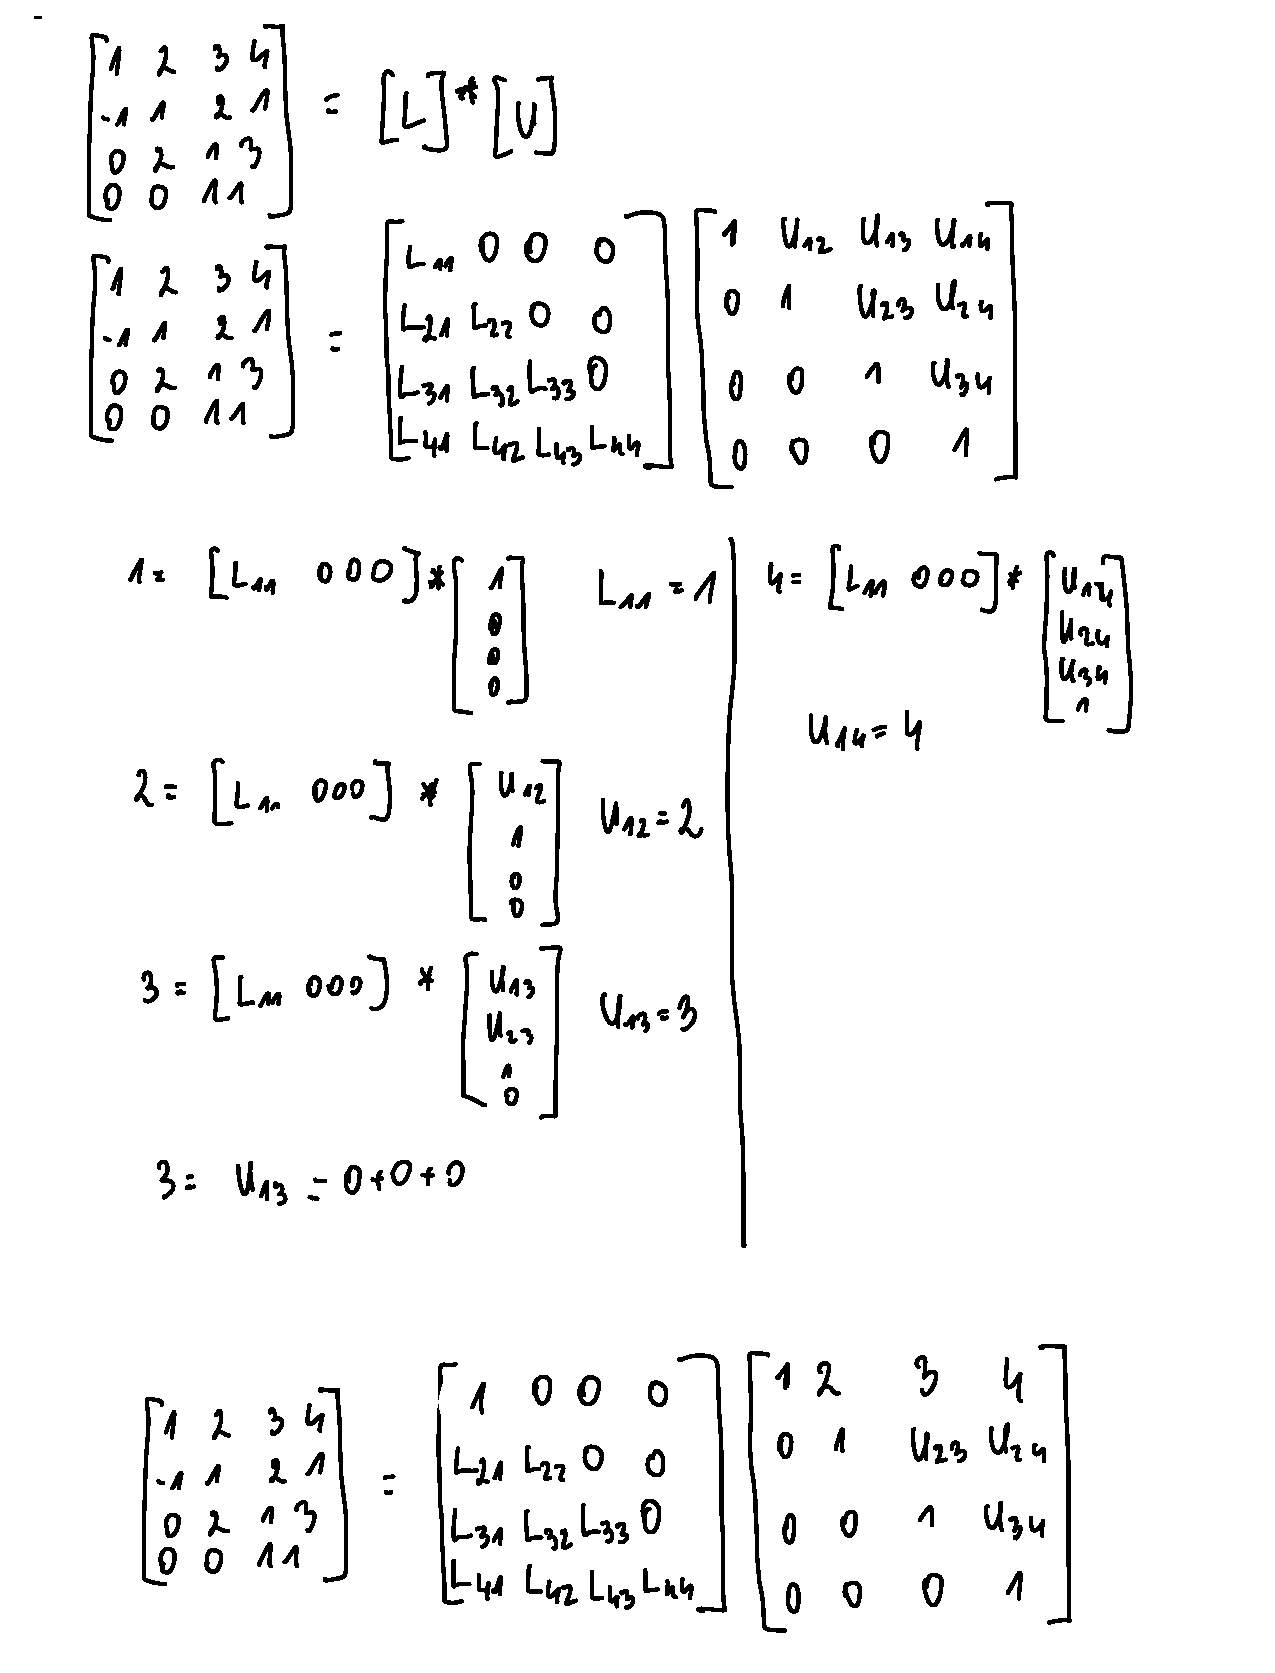
\includepdf[pages=-]{zad5.pdf}
\section{Zadanie nr. 6}
fiki miki maka paka

\[
  \centering
  \linespread{2}\selectfont
  \addtolength{\arraycolsep}{10pt}
 \begin{gmatrix}[b]
  1 & 2 & 2 & 3 & 1\\
  2 & 4 & 4 & 6 & 2\\
  3 & 6 & 6 & 9 & 6\\
  1 & 2 & 4 & 5 & 3 
 \rowops
 \add[-2]01
 \add[-3]02
 \add[-1]03
\end{gmatrix}
\]
\[
  \centering
  \linespread{2}\selectfont
  \addtolength{\arraycolsep}{10pt}
 \begin{gmatrix}[b]
  1 & 2 & 2 & 3 & 1\\
  0 & 0 & 0 & 0 & 0\\
  0 & 0 & 0 & 0 & 3\\
  0 & 0 & 2 & 2 & 2 
 \rowops
 \swap13
\end{gmatrix}
\]
\[
  \centering
  \linespread{2}\selectfont
  \addtolength{\arraycolsep}{10pt}
 \begin{gmatrix}[b]
  1 & 2 & 2 & 3 & 1\\
  0 & 0 & 2 & 2 & 2\\
  0 & 0 & 0 & 0 & 3\\
  0 & 0 & 0 & 0 & 0
 \rowops
 \mult{1}{\cdot \left(\frac1{2}\right)}
 \mult{2}{\cdot \left(\frac1{3}\right)}
\end{gmatrix}
\]
\[
  \centering
  \linespread{2}\selectfont
  \addtolength{\arraycolsep}{10pt}
 \begin{gmatrix}[b]
  1 & 2 & 2 & 3 & 1\\
  0 & 0 & 1 & 1 & 1\\
  0 & 0 & 0 & 0 & 1\\
  0 & 0 & 0 & 0 & 0
 \rowops
\add[-2]10
\add20
\add[-1]21
\end{gmatrix}
\]
\[
  \centering
  \linespread{2}\selectfont
  \addtolength{\arraycolsep}{10pt}
 \begin{gmatrix}[b]
  1 & 2 & 0 & 1 & 0\\
  0 & 0 & 1 & 1 & 0\\
  0 & 0 & 0 & 0 & 1\\
  0 & 0 & 0 & 0 & 0
\end{gmatrix}
\]

cimicirimci

\section{Zadanie nr. 7}

place your code here

\section{Zadanie nr. 8}

place your code here

\section{Zadanie nr. 9}
równania
mpo

\[ \begin{bmatrix}
  \centering
  \linespread{2}\selectfont
  \addtolength{\arraycolsep}{10pt}
  0 & 0 & R & 0 & R & 0\\
  0 & 0 & -R & R & 0 & 0\\
  0 & 0 & 0 & 0 & R & -R\\
  -1 & 0 & 1 & 1 & 0 & 0\\
  0 & 1 & 1 & 0 & -1 & 0\\
  0 & 1 & 0 & -1 & 0 & 1\\

\end{bmatrix}
\times
\begin{bmatrix}
  I_{1}\\
  I_{2}\\ 
  I_{3}\\ 
  I_{4}\\ 
  I_{5}\\ 
  I_{6}\\ 
\end{bmatrix}
=
\begin{bmatrix}
  E_{1}\\
  E_{2}\\ 
  E_{3}\\ 
  0\\ 
  0\\ 
  0\\ 
\end{bmatrix} \]

\[
  \centering
  \linespread{2}\selectfont
  \addtolength{\arraycolsep}{10pt}
 \begin{gmatrix}[b]
  0 & 0 & 20 & 0 & 20 & 0 & \BAR & 20\\
  0 & 0 & -20 & 20 & 0 & 0 & \BAR & 10\\
  0 & 0 & 0 & 0 & 20 & -20 & \BAR & 10\\
  -1 & 0 & 1 & 1 & 0 & 0 & \BAR & 0\\
  0 & 1 & 1 & 0 & -1 & 0 & \BAR & 0\\
  0 & 1 & 0 & -1 & 0 & 1 & \BAR & 0
  \rowops
  \swap03
  \swap14
  \swap25
\end{gmatrix}
\]

\[
  \centering
  \linespread{2}\selectfont
  \addtolength{\arraycolsep}{10pt}
 \begin{gmatrix}[b]
  -1 & 0 & 1 & 1 & 0 & 0 & \BAR & 0\\
  0 & 1 & 1 & 0 & -1 & 0 & \BAR & 0\\
  0 & 1 & 0 & -1 & 0 & 1 & \BAR & 0\\
  0 & 0 & 20 & 0 & 20 & 0 & \BAR & 20\\
  0 & 0 & -20 & 20 & 0 & 0 & \BAR & 10\\
  0 & 0 & 0 & 0 & 20 & -20 & \BAR & 10
  \rowops
  \add[-1]12
\end{gmatrix}
\]

\[
  \centering
  \linespread{2}\selectfont
  \addtolength{\arraycolsep}{10pt}
 \begin{gmatrix}[b]
  -1 & 0 & 1 & 1 & 0 & 0 & \BAR & 0\\
  0 & 1 & 1 & 0 & -1 & 0 & \BAR & 0\\
  0 & 0 & -1 & -1 & 1 & 1 & \BAR & 0\\
  0 & 0 & 20 & 0 & 20 & 0 & \BAR & 20\\
  0 & 0 & -20 & 20 & 0 & 0 & \BAR & 10\\
  0 & 0 & 0 & 0 & 20 & -20 & \BAR & 10
  \rowops
  \add[20]23
  \add[-20]24
\end{gmatrix}
\]

\[
  \centering
  \linespread{2}\selectfont
  \addtolength{\arraycolsep}{10pt}
 \begin{gmatrix}[b]
  -1 & 0 & 1 & 1 & 0 & 0 & \BAR & 0\\
  0 & 1 & 1 & 0 & -1 & 0 & \BAR & 0\\
  0 & 0 & -1 & -1 & 1 & 1 & \BAR & 0\\
  0 & 0 & 0 & -20 & 40 & 20 & \BAR & 20\\
  0 & 0 & 0 & 40 & -20 & -20 & \BAR & 10\\
  0 & 0 & 0 & 0 & 20 & -20 & \BAR & 10
  \rowops
  \add[2]34
\end{gmatrix}
\]

\[
  \centering
  \linespread{2}\selectfont
  \addtolength{\arraycolsep}{10pt}
 \begin{gmatrix}[b]
  -1 & 0 & 1 & 1 & 0 & 0 & \BAR & 0\\
  0 & 1 & 1 & 0 & -1 & 0 & \BAR & 0\\
  0 & 0 & -1 & -1 & 1 & 1 & \BAR & 0\\
  0 & 0 & 0 & -20 & 40 & 20 & \BAR & 20\\
  0 & 0 & 0 & 0 & 60 & 20 & \BAR & 50\\
  0 & 0 & 0 & 0 & 20 & -20 & \BAR & 10
  \rowops
  \add[-\frac1{3}]45
\end{gmatrix}
\]

\[
  \centering
  \linespread{2}\selectfont
  \addtolength{\arraycolsep}{10pt}
 \begin{gmatrix}[b]
  -1 & 0 & 1 & 1 & 0 & 0 & \BAR & 0\\
  0 & 1 & 1 & 0 & -1 & 0 & \BAR & 0\\
  0 & 0 & -1 & -1 & 1 & 1 & \BAR & 0\\
  0 & 0 & 0 & -20 & 40 & 20 & \BAR & 20\\
  0 & 0 & 0 & 0 & 60 & 20 & \BAR & 50\\
  0 & 0 & 0 & 0 & 0 & -\frac{80}{3} & \BAR & -\frac{20}{3}
\end{gmatrix}
\]

tego typu benc benc

\section{Wnioski}
Zgodnie z obliczeniami wyniki obliczeń zostały wykonane prawidłowo
\end{document} 